Information has usually been referred to as one of the key aspects that every learning system needs in order to increase its capabilities and improve its performance. This is especially relevant for the Data Analytics field and the process of designing machine learning applications, where many experts usually refer to information as a powerful metric to indicate the success of their architecture at solving a particular problem. Due to the plethora of works already available online to master and use different techniques, the goal of this work is to asses the capabilities of these techniques and discuss its informational properties. 

%\setlength{\parindent}{10ex}

During the last few years, the topic of Big Data has become increasingly more important in our society. It is currently being used or developed in almost every industry in the world\footnote{(Quote article to reinforce my position on this matter? {\color{red} FVA: YES!})} and it is growing faster every day. While methods like Deep Neural Networks are beginning to be widespread available,  researchers tend to use the same approaches and steps to get their results. Rather than trying new methods, it is an industry standard to use a certain set of techniques when presented with a type of problem and then to try to optimise them. It is just assumed that these methods are powerful enough to find a suitable answer. 

An instance of this model can be found in Figure~\ref{fig:fig1}.\subref{fig:fig1b}, where each block represents a different function inside an end-to-end informational model. We can only take measures outside each of the blocks and the contents or the methods being used inside are outside of the scope of the task. By not being able to access each one of the blocks to evaluate the processes happening inside of them, we may only fix or change their inputs to try to improve our results.
%
\begin{figure}[h]
\begin{subfigure}{1\textwidth}  
 \centering
  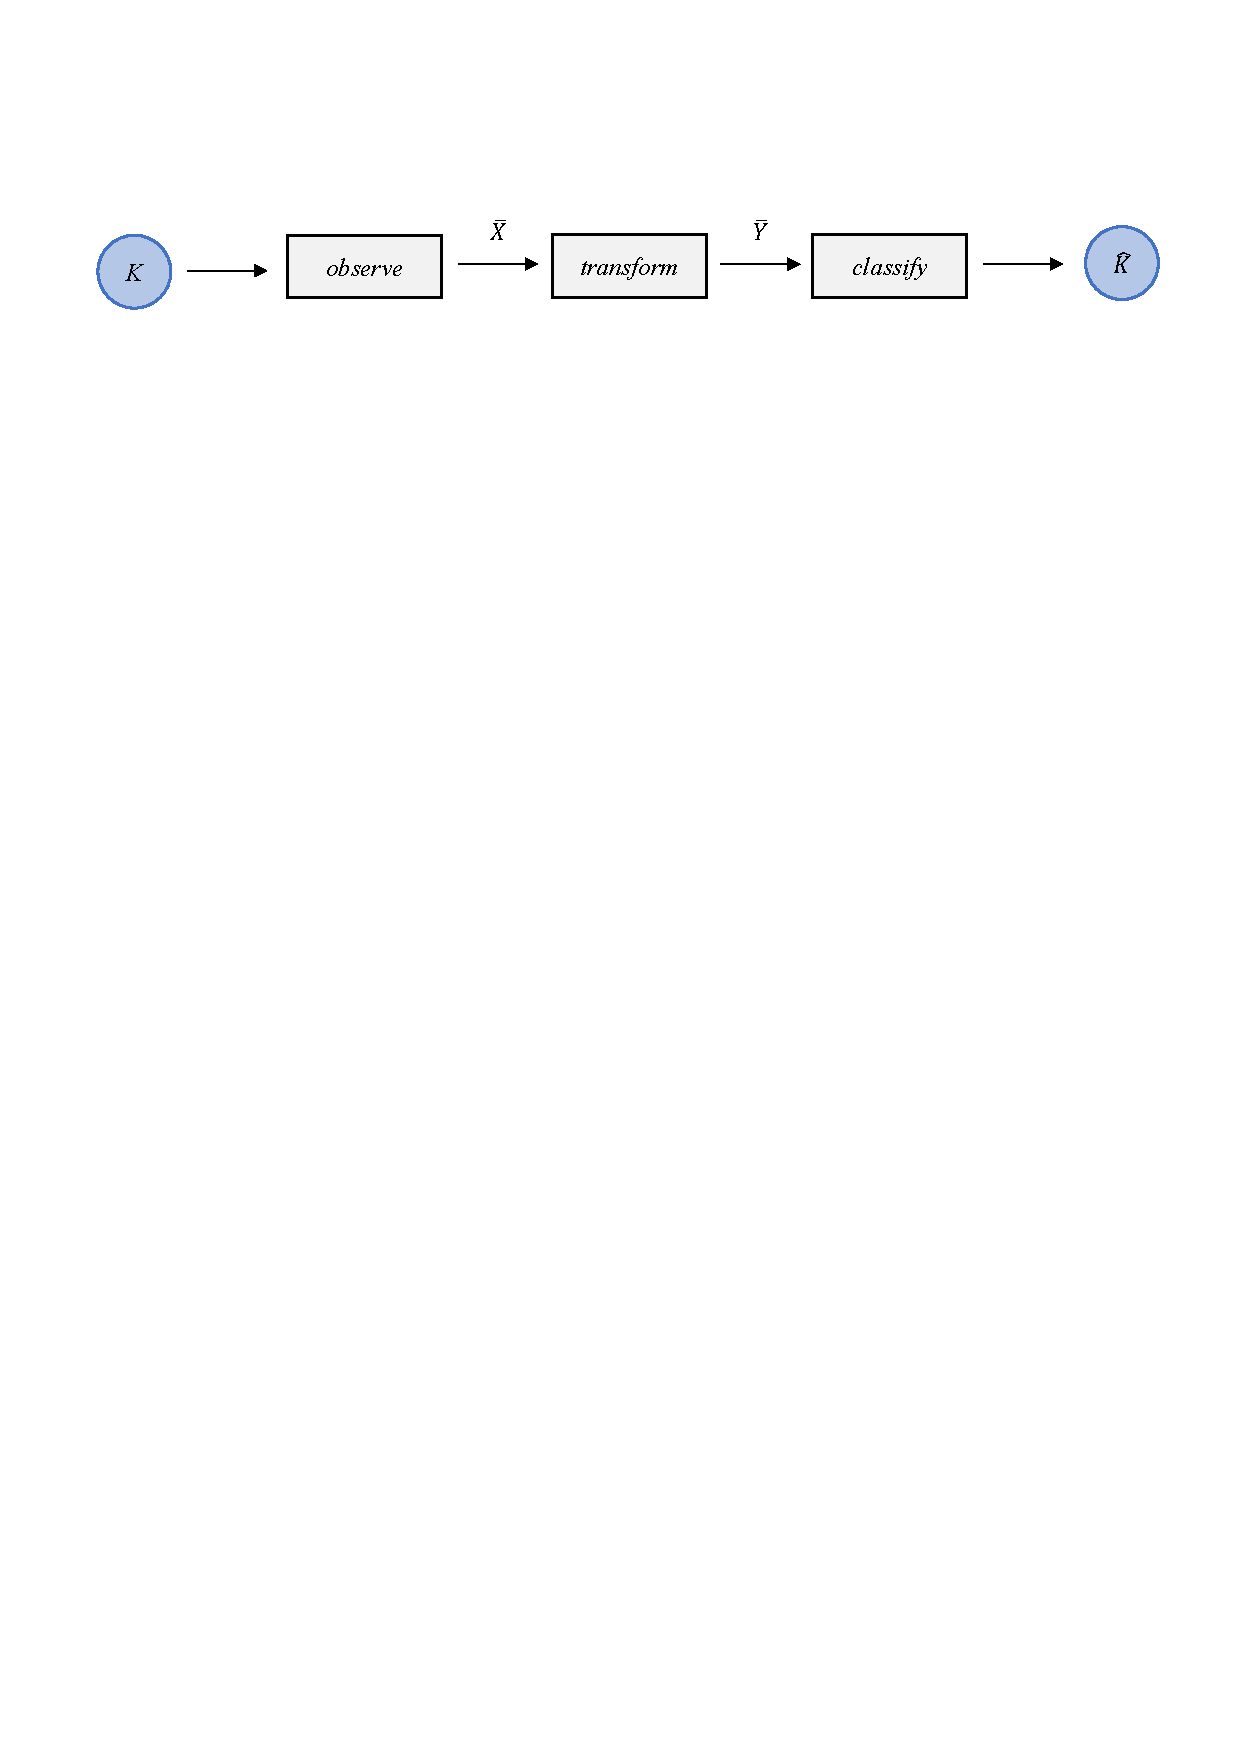
\includegraphics[width=16cm]{Figuras_tfg/Figura1_tfg}
  \caption{Conceptual representation of a classification process mimicking a communication scheme of boxes.}
 \label{fig:fig1b} 
\end{subfigure}%  

\begin{subfigure}{1\textwidth} 
  \centering
  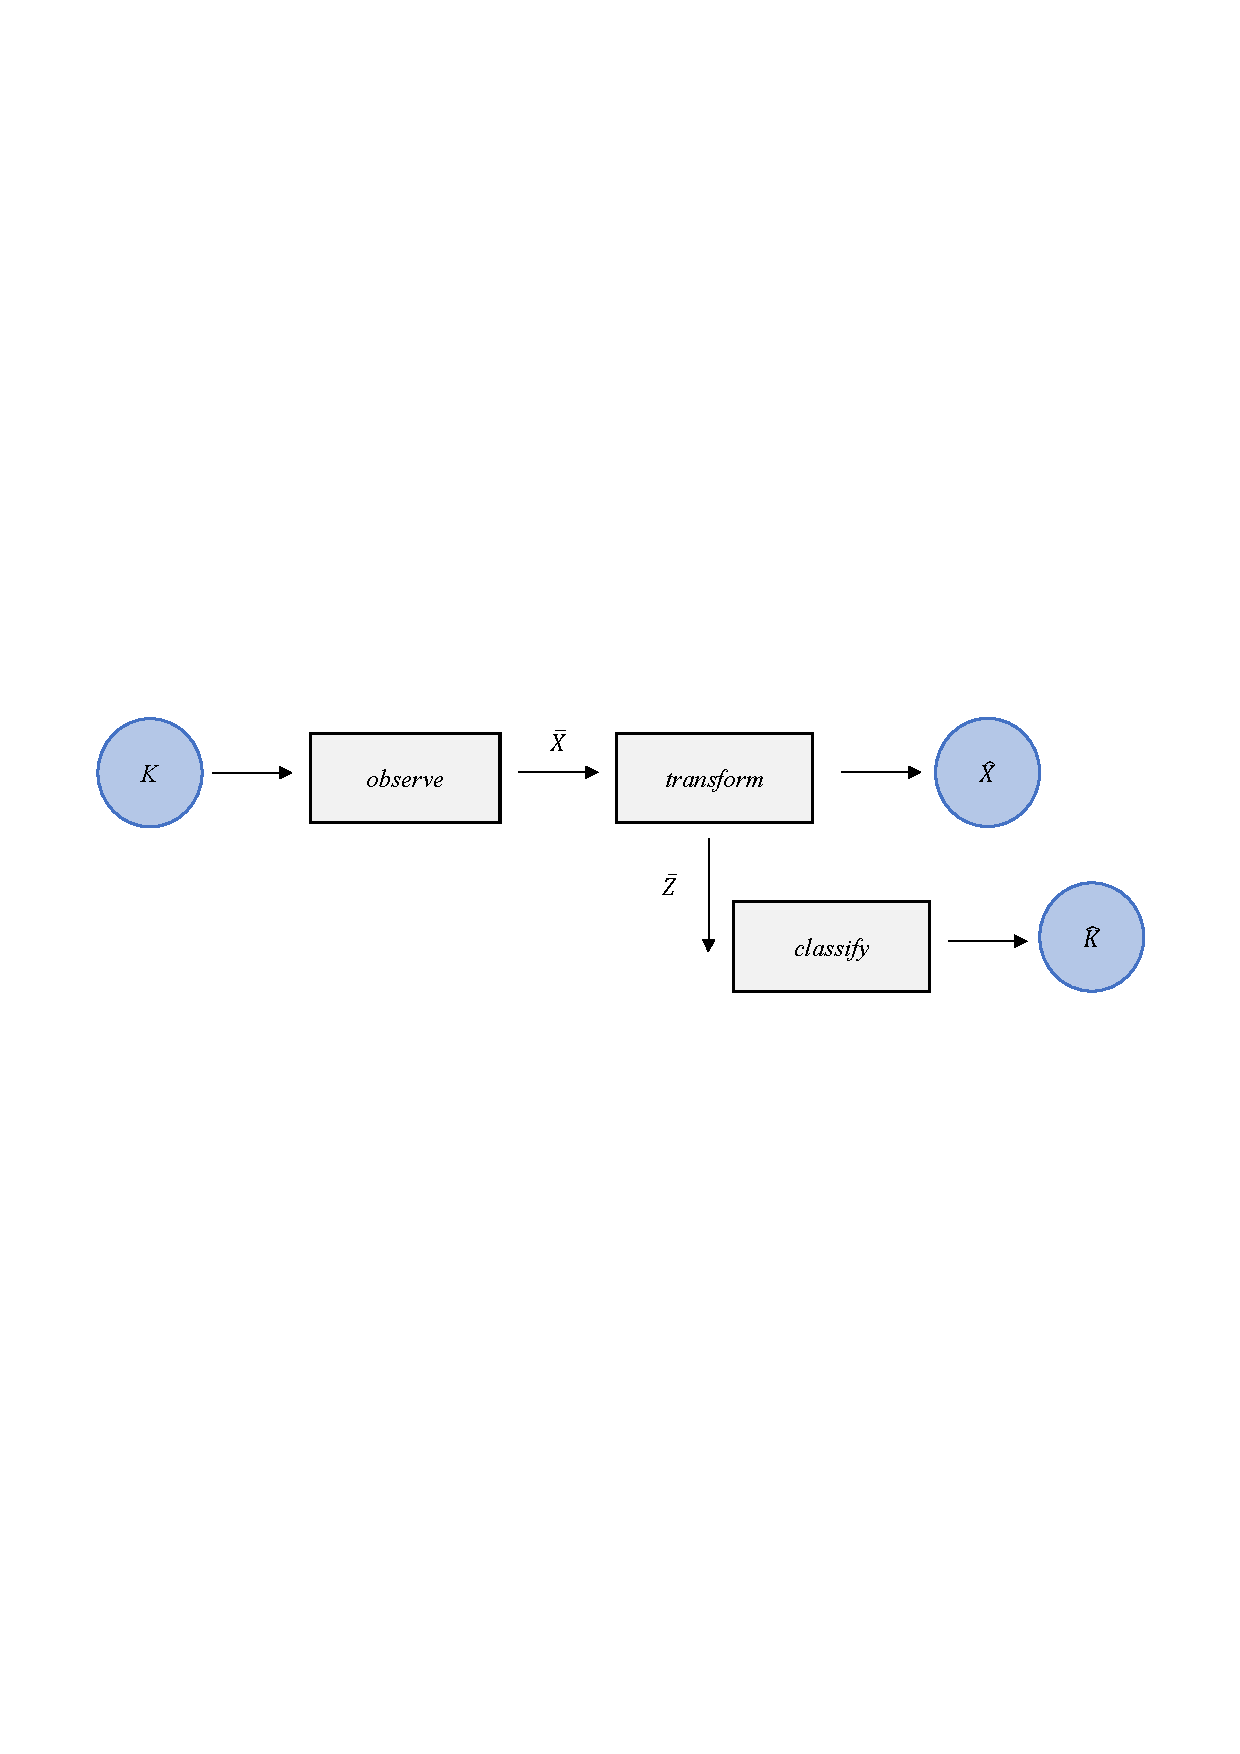
\includegraphics[width=16.5cm]{Figuras_tfg/Figura1_1_tfg}
  \caption{Our end-to-end scheme uses the information regarded from inside the transformation block and we then produce two outputs. First, the predicted (X) which we can use to measure our transformation accuracy. Secondly, the (Z), which contains compressed information about (X)}
  \label{fig:fig1a} 
\end{subfigure}%  
\caption{Comparison between the classical view of a supervised classification in (a) versus the the model implemented for the purpose of this work in (b).}
\label{fig:fig1}
\end{figure}


The model that I will be implementing will be an adaptation of the scheme on Figure~\ref{fig:fig1}.\subref{fig:fig1a}. To further investigate on the boundaries of Information transmission , I will be using an \textbf{Autoencoder} to test the Information Bottleneck Principle~\cite{refToInfBottleNeck}. 

%FVA: find the original paper of the IB principle, for instance in Wikipedia, and cite it here.  The bibliography has to go in its own *.bib file.
%I am including one with the same name as the main file, with the papers on the triangles, which I can very easily create from my reference manager. You just have to add to this one with a bib manager. I use BibDesk which comes along with TeXStudio.
% You have to cite the papers on the triangles in the triangles section, of course. 

In this report, I designed the following model which provides reliable information about the process of data compression and the limits of quantifiable information:

% FVA: itemizations and enumerations have their own enviroments in LaTeX.
\begin{itemize}
\item  We have a random source $K$ generating observations. Through a process of measurements, our system then will be provided with other random observations $\hat{X}$. 

\item The output observations  are then fed to the Autoencoder, which will then reduce the $\overline X$ (X con gorro) into another vector $Z$ with a different length but retaining the information from the input vector in a compressed from. 

\item The Autoencoder also provides  an output, which should be a reconstruction of the observations used to feed the Deep Learning structure. 

\item The $\overline Z$ is then used for the classifying task of choice to output the predicted labels. 

\end{itemize}

Note that Figure~\ref{ifg:fig1a} follows a similar model to that of Figure \ref{ifg:fig1}, but its transformation block is used to access the inside content of it rather than to provide a typical representation of an end-to-end transformation scheme. Although both of them typify a MIMO (Multiple Input Multiple Output) block, the Autoencoder is essentially an unsupervised transformation method, while the transformation block can be either composed by supervised or unsupervised task. The inner workings and different features of the Autoencoder will be explained on Section 2.1. \par

% FVA: this is a reading aid, well done! Now you also need to tell what the rest of the chapters are. 
Next is a review r the concepts to be used on this Final Degree Project and the rest of methods to use on it.
